This graduation work aims to discuss the main maze exploration algorithms and then propose a method where multi-agents must find the maze solution without any type of communication, only working with probability distributions to guide their behaviors. The main challenge of this research is to find a distributed exploration approach with total communication restriction since an agent's partial knowledge cannot be shared with another agent and, at the same time, a single agent must avoid repeating a branch of another agent. The proposed maze structure abstraction is a traditional regular grid that can be generalized into graphs.

This report is the initial part of the bachelor's thesis, and this chapter intends to introduce the general concept of the related thesis and present the motivation (Section \ref{section_intro_motivation}), the related work (Section \ref{section_intro_relatedwork}), and the main definitions about maze-solving algorithms (Section \ref{section_intro_definitions}).

\section{Motivation}
\label{section_intro_motivation}
Graph exploration has been the target of studies since Leonhard Euler proved that Seven Bridges of K�nigsberg \cite{ShieldsR2012} has no solution. It has been researched not only in academia but also in the industry due to several practical applications, like airline scheduling, planning path on maps, search engine algorithms, social media marketing, Internet routing protocols, and robotics.

Specifically in robotics, graph exploration can be used to explore a maze with a single agent through a bunch of traditional algorithms: random mouse, wall follower, Tr�maux, etc \cite{Sadik2010}. And it can be useful to guide many real-life problems such as search in nuclear plant disasters, burning buildings, and extraterrestrial environments. In these previous examples, the multi-agent exploration is more interesting than the single-agent approach since it can speed up the exploration. Recent studies have explored multi-agent maze-solving algorithms as seen in the Multi-Agent Maze Exploration paper \cite{KivelevitchCohen2010}, where authors proposed a Tarry's algorithm generalization. It is important to emphasize that maze-solving algorithms consider that the structure is unknown, and then traditional search algorithms, such as Dijkstra and A*, cannot be used to solve the maze.

Traditional multi-agent maze exploration approaches is based on internal communication between agents, where each agent knows about visited cells by another agent. It avoids a second exploration in a useless path and thus it decreases computational costs. However, there are some real situations where communication is limited or impossible, such as deep sea exploration, search in large wall structures, or search with low energy-based autonomous agents. 

However, the incommunicable approach between agents have not been concretely found in the literature despite it may have real applications and may guide search plans in real-world problems. In order to explore it, this work presents some ways to achieve the maze solution based on agents without communication, that might be generalized to graph exploration algorithms.

\section{Related work}
\label{section_intro_relatedwork}
RELATED WORK

\section{Definitions}
\label{section_intro_definitions}
DEFINITIONS

%\section{Exemplo}
%\begin{figure}[ht!]
%\centering
%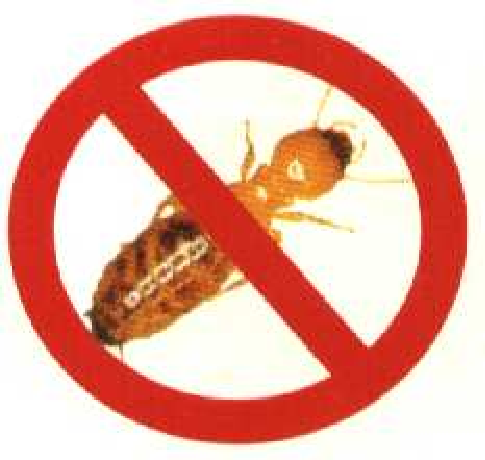
\includegraphics[width=0.5\textwidth]{Cap1/cupim}
%\caption{Proibido estacionar cupins. Legenda grande, com o objetivo de demonstrar a indenta��o na lista de figuras.}
%\label{cupim}
%\end{figure}

%\begin{table}
%\caption{Exemplo de uma Tabela}
%\label{minhatab}
%\center
%\begin{tabular}{cccc}
  % after \\: \hline or \cline{col1-col2} \cline{col3-col4} ...
 % \hline
%	Par�metro & Unidade & Valor da simula��o & Valor experimental   \\
%	\hline
 % Comprimento, $\alpha$ & $m$ &  $8,23$  & $8,54$ \\
 % Altura, $\beta$ & $m$     &  $29,1$ & $28,3$\\
%	Velocidade, $v$ & $m/s$  &  $60,2$ & $67,3$\\
%	\hline
%\end{tabular}
%\end{table}
